\documentclass{article}
\usepackage{graphicx} % Required for inserting images

\title{IMMAGINI E RIFLESSIONI TESI}
\author{bignozzi.1855163 }
\date{September 2024}

\begin{document}

\maketitle

\section{GRAFO}
Allora la scelta per il grafo, per semplicità di scrittura è stato quello di fare dei legami solo e solo se il raggio di interazione è minor edi un certo valore. Come si fa a trovare la teshold migliroe per il raggio in quesot modello?
Si runna il modello al fine di minimizzare i MAE sui residui ogni volta ocn un raggio diverso. Il modello che ottiene il mae min,ore è quello che meglio descrive il tutto.
Inoltre in questo modo è possibile ottenre anche il miglior grafo senza alcun tipo di vincolo.
Prima di predirre i beta factor per davvero (con autovalori e autovettori) avrei bisogno di utilizzare i parametri corretti epr temperatura Kb ecc.

\section{Matrice di kirchoff}
La matrice di Kirchhoff (o laplaciana) rappresenta un'analogia con una rete elastica in cui le connessioni tra i nodi (atomi) descrivono le interazioni elastiche. Questa matrice codifica il modo in cui ogni nodo è collegato agli altri, e attraverso i suoi autovalori e autovettori, si può studiare come le vibrazioni collettive (modi normali) si propagano attraverso il sistema.
Autovalori e autovettori della matrice di Kirchhoff:
Gli autovalori della matrice di Kirchhoff descrivono le frequenze naturali di vibrazione del sistema.
Gli autovettori rappresentano i corrispondenti modi normali di vibrazione, cioè come ogni nodo (atomo) si muove in un determinato modo di vibrazione.
Quelli a bassa frequenza corrispondono alle vibrazioni collettive del sistema, quelli ad alta frequenza sono fluttuazioni locali 
% Inserisci la prima immagine
\section{Calcolo correlazione}
Risolvi l'equazione differenziale:
\begin{equation}
    \gamma \dot{x}_i = -g \sum_j K_{ij} x_j + \sqrt{2 \gamma k_B T} \xi_i(t)
    \end{equation}
    
\begin{equation}
    \mathbf{x}(t) = e^{-\mu K t} \left\{ \mathbf{x}(0) + \sqrt{\frac{2k_B T}{\gamma}} \int_0^t ds \, e^{-\mu K s} \xi(s) \right\}
    \end{equation}
\begin{equation}
    C(t) = \langle \mathbf{x}(0) \mathbf{x}^\top(t) \rangle
    \end{equation}
\begin{equation}
    C(t) = e^{-\mu \mathbf{K} t} C(0)
    \end{equation}
        
\begin{equation}
    C(0) = \langle \mathbf{x}(0) \mathbf{x}^\top(0) \rangle
    \end{equation}
\begin{equation}
    \mathbf{K} = \mathbf{U} \Lambda \mathbf{U}^\dagger
    \end{equation}
        
\begin{equation}
    C_{ij}(t) = \frac{3 k_B T}{g} \sum_{k=2}^{N} \frac{u_i(k) u_j(k)}{\lambda(k)} e^{-\lambda(k) t}
    \end{equation}
        
\section{Calcolo risposta}
\begin{equation}
    R(t) = \frac{C(t)}{C(0)}
    \end{equation}
\begin{equation}
    \mathbf{R}(t) = e^{-\mu \mathbf{K} t}
    \end{equation}
\begin{equation}
    R_{ij}(t) = - \left\langle \frac{\partial \ln P_s(x)}{\partial x_j(t)} x_i(0) \right\rangle
    \end{equation}
\begin{equation}
    R_{ij}(t) = \sum_{k=1}^{N} u_i(k) u_j(k) e^{-\lambda(k) t}
    \end{equation}






images/2m10Residual Correlation C_ij for i=22 as a function of j at time index 0.png
\section{2M0Z}
\begin{figure}[h]
    \centering
    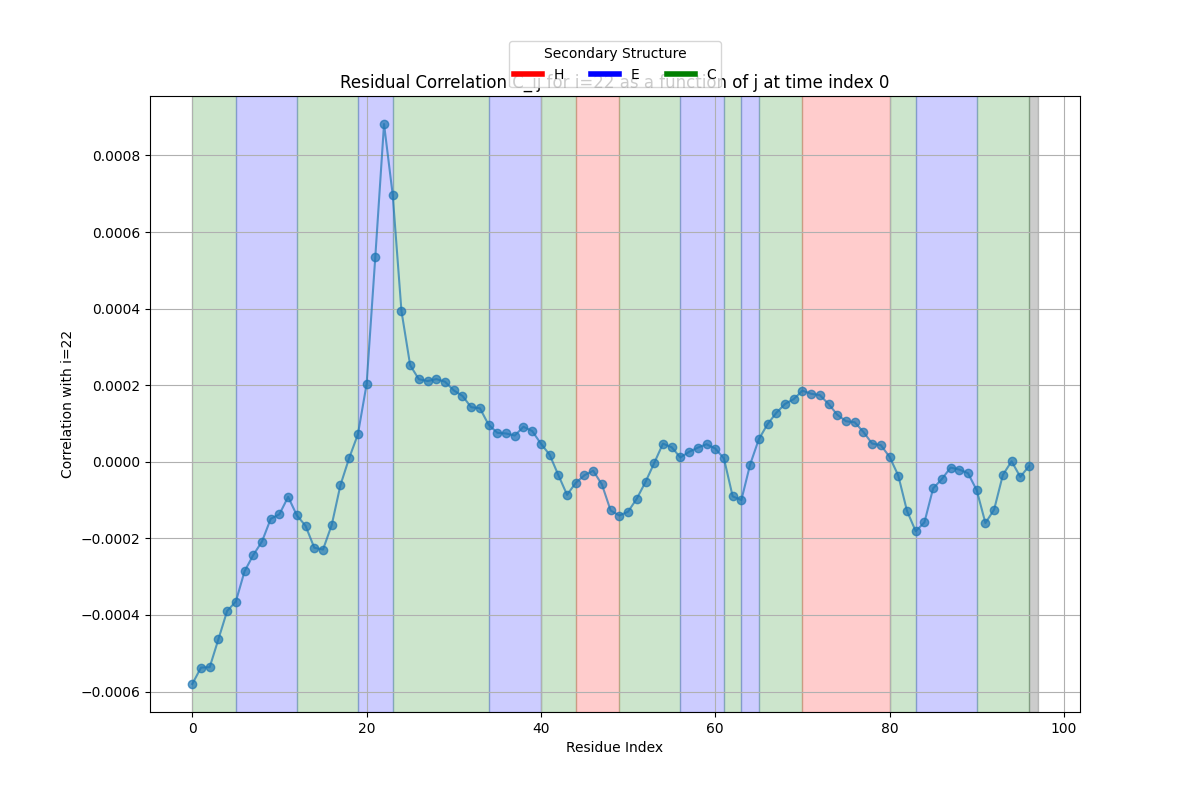
\includegraphics[width=0.5\textwidth]{images/2m0zResidual Correlation C_ij for i=22 as a function of j at time index 0.png}
    \caption{Correlazione}
\end{figure}
\begin{figure}[h]
    \centering
    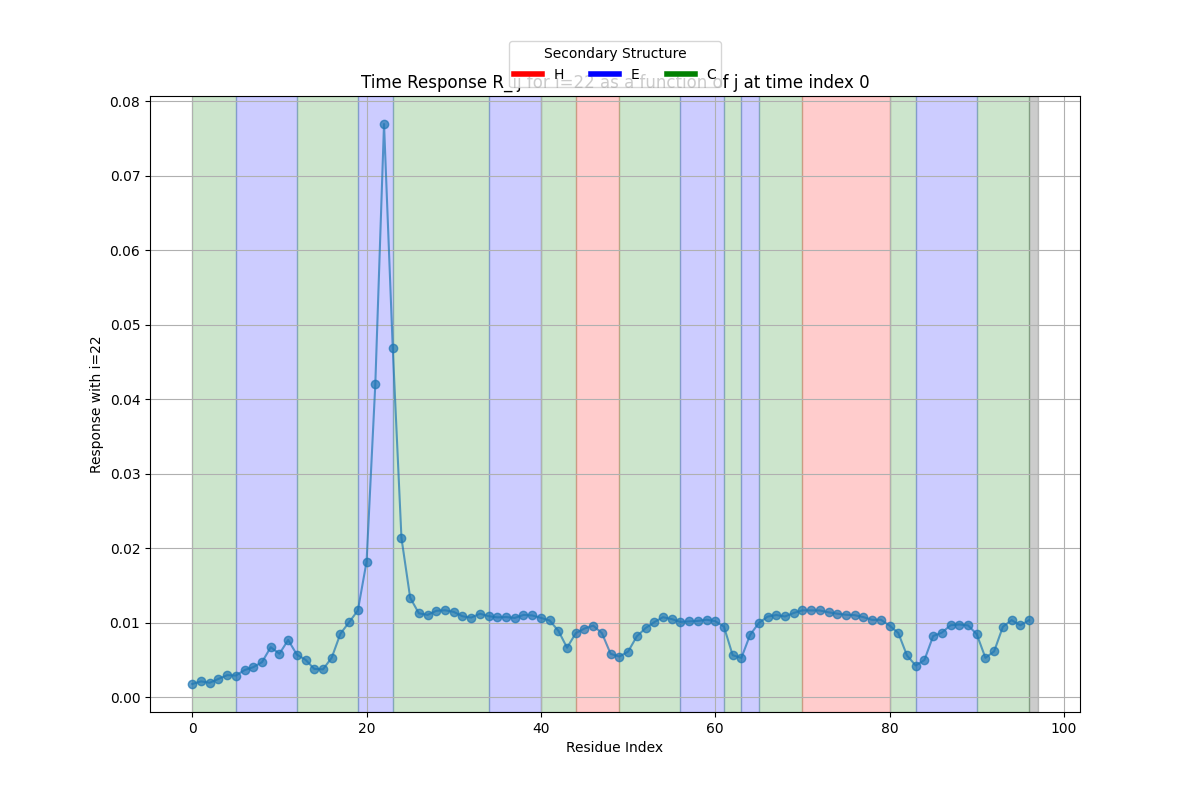
\includegraphics[width=0.5\textwidth]{images/2m0zTime Response R_ij for i=22 as a function of j at time index 0.png}
    \caption{Risposta}
\end{figure}

\begin{figure}[h]
    \centering
    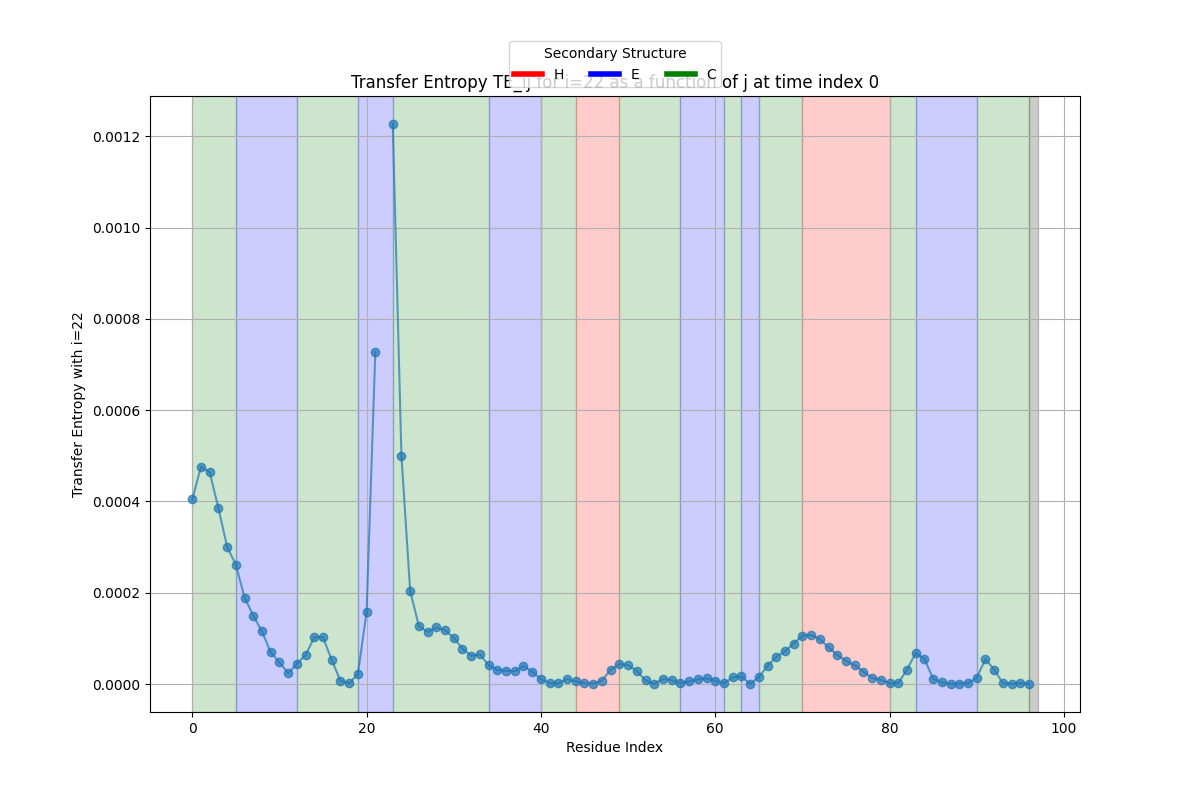
\includegraphics[width=0.5\textwidth]{images/2m0zTransfer Entropy TE_ij for i=22 as a function of j at time index 0.png}
    \caption{Transfer Entropy}
\end{figure}

\section{2M10}
\begin{figure}[h]
    \centering                            
                                           
    
    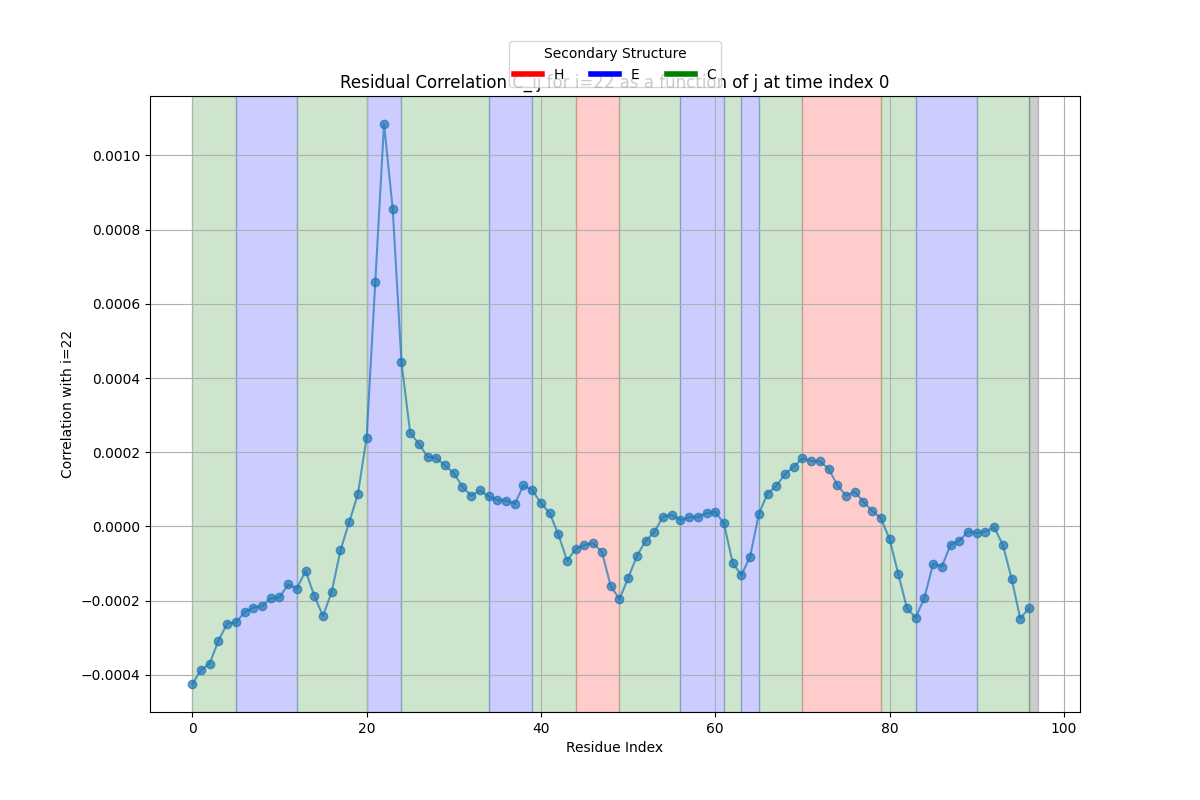
\includegraphics[width=0.5\textwidth]{images/2m10Residual Correlation C_ij for i=22 as a function of j at time index 0.png}
    \caption{Correlazione}
\end{figure}
\begin{figure}[h]
    \centering
    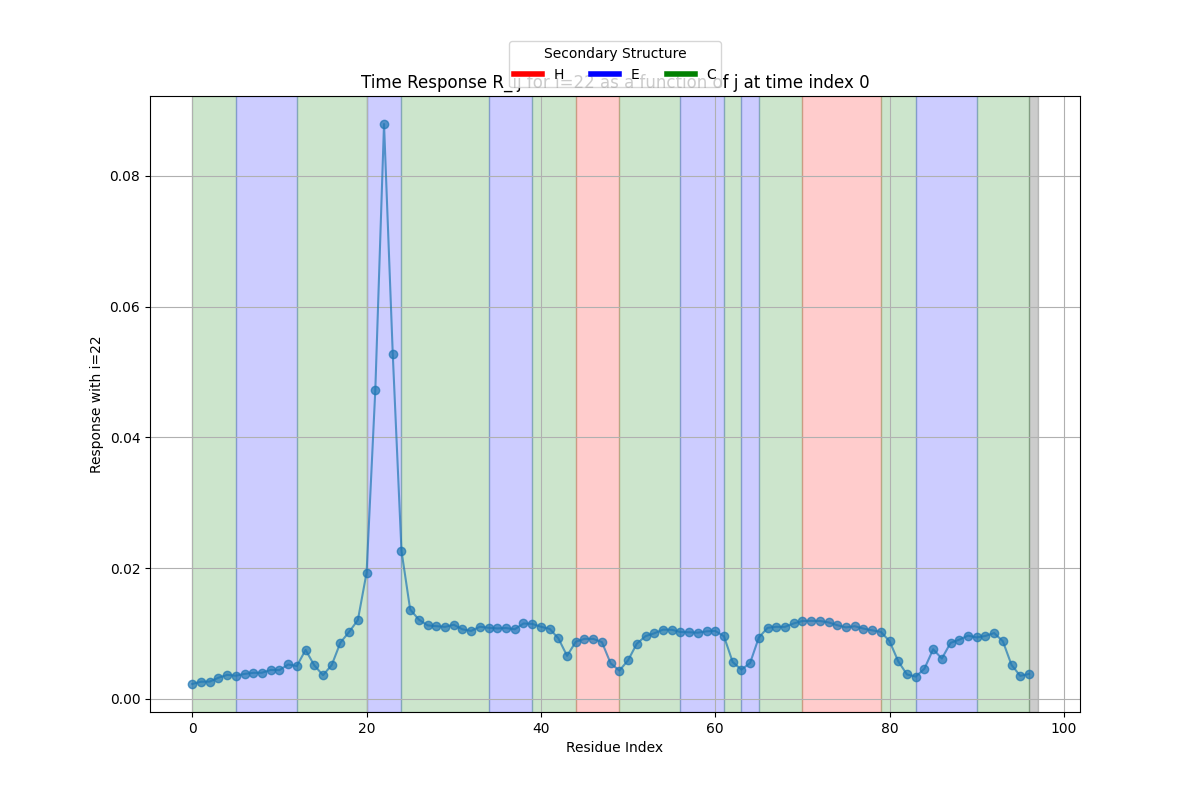
\includegraphics[width=0.5\textwidth]{images/2m10Time Response R_ij for i=22 as a function of j at time index 0.png}
    \caption{Risposta}
\end{figure}

\begin{figure}[h]
    \centering
    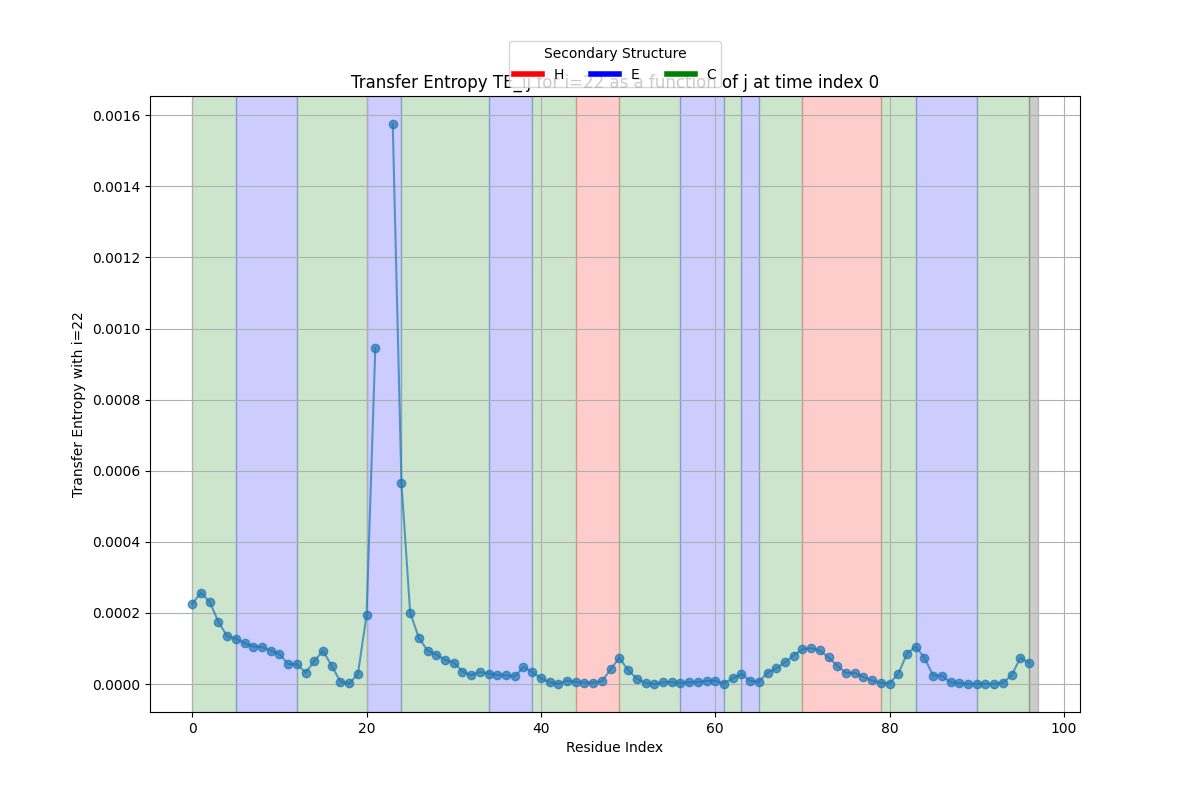
\includegraphics[width=0.5\textwidth]{images/2m10Transfer Entropy TE_ij for i=22 as a function of j at time index 0.png}
    \caption{Transfer Entropy}
\end{figure}
\section{3LNX}
\begin{figure}[h]
    \centering
    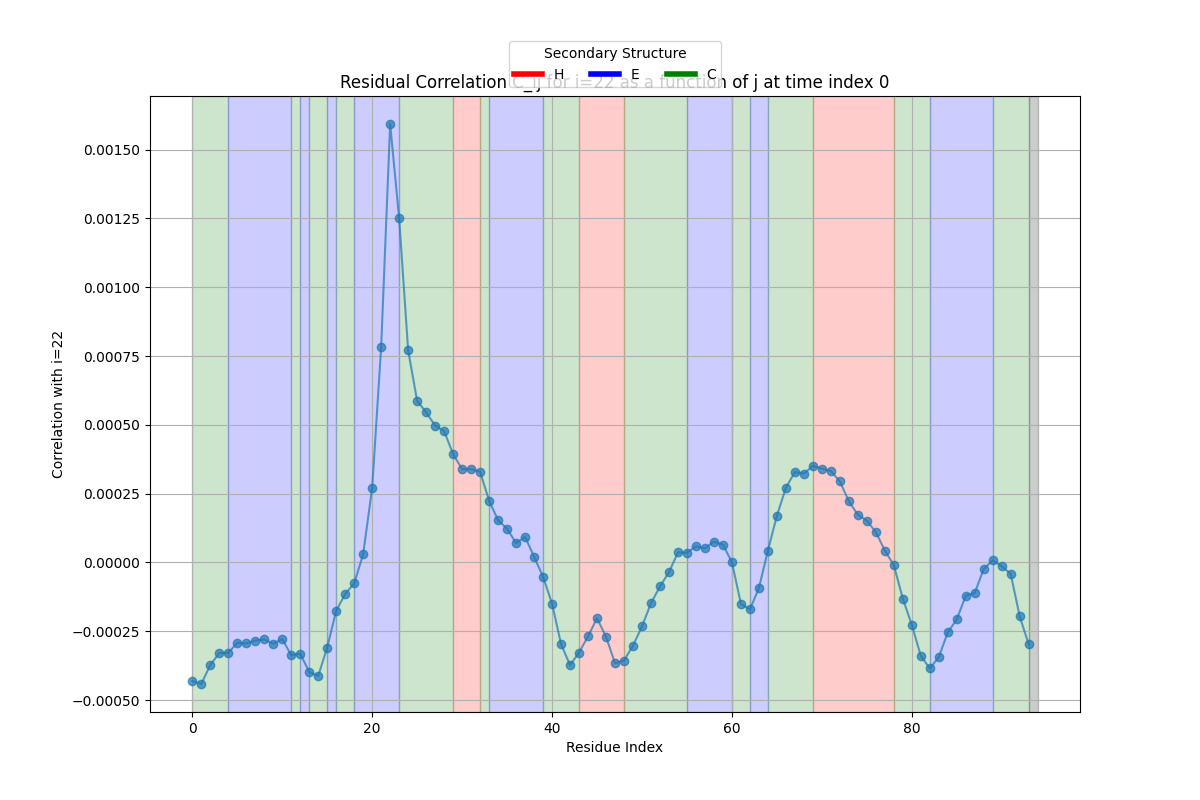
\includegraphics[width=0.5\textwidth]{images/3LNXResidual Correlation C_ij for i=22 as a function of j at time index 0.png}
    \caption{Correlazione}
\end{figure}
\begin{figure}[h]
    \centering
    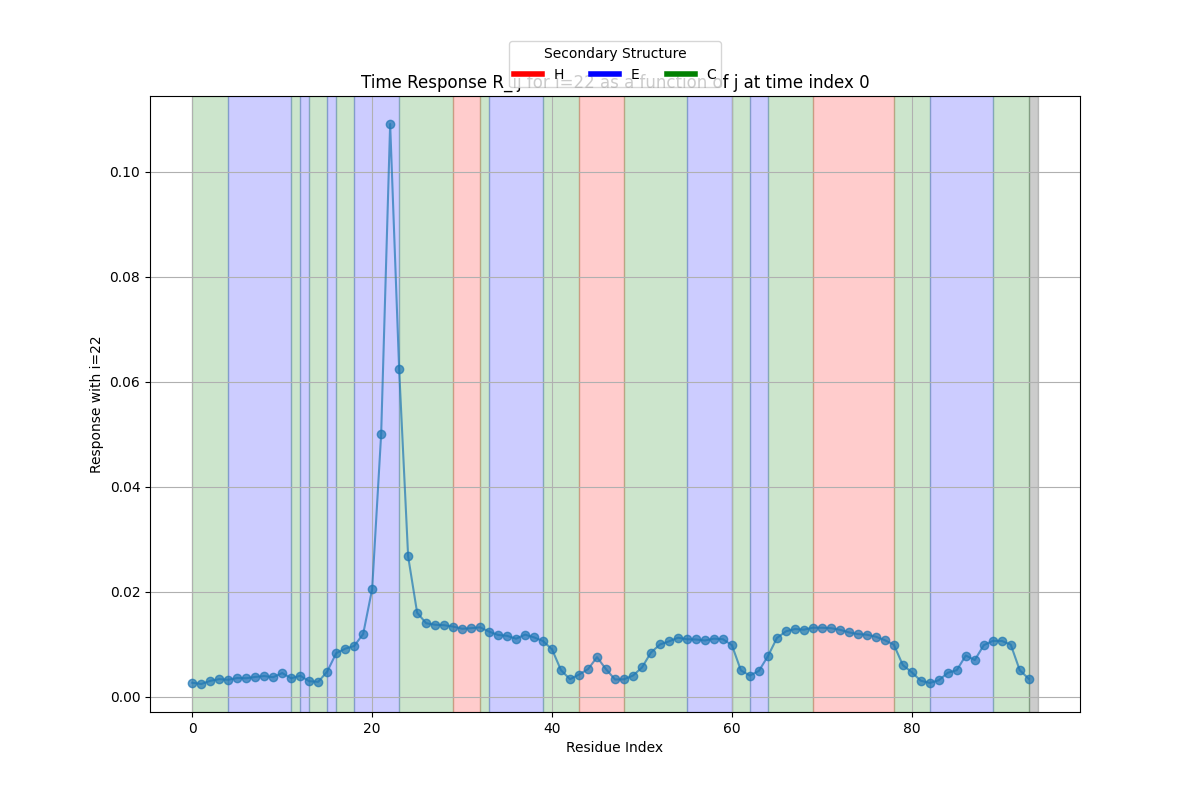
\includegraphics[width=0.5\textwidth]{images/3LNXTime Response R_ij for i=22 as a function of j at time index 0.png}
    \caption{Risposta}
\end{figure}

\begin{figure}[h]
    \centering
    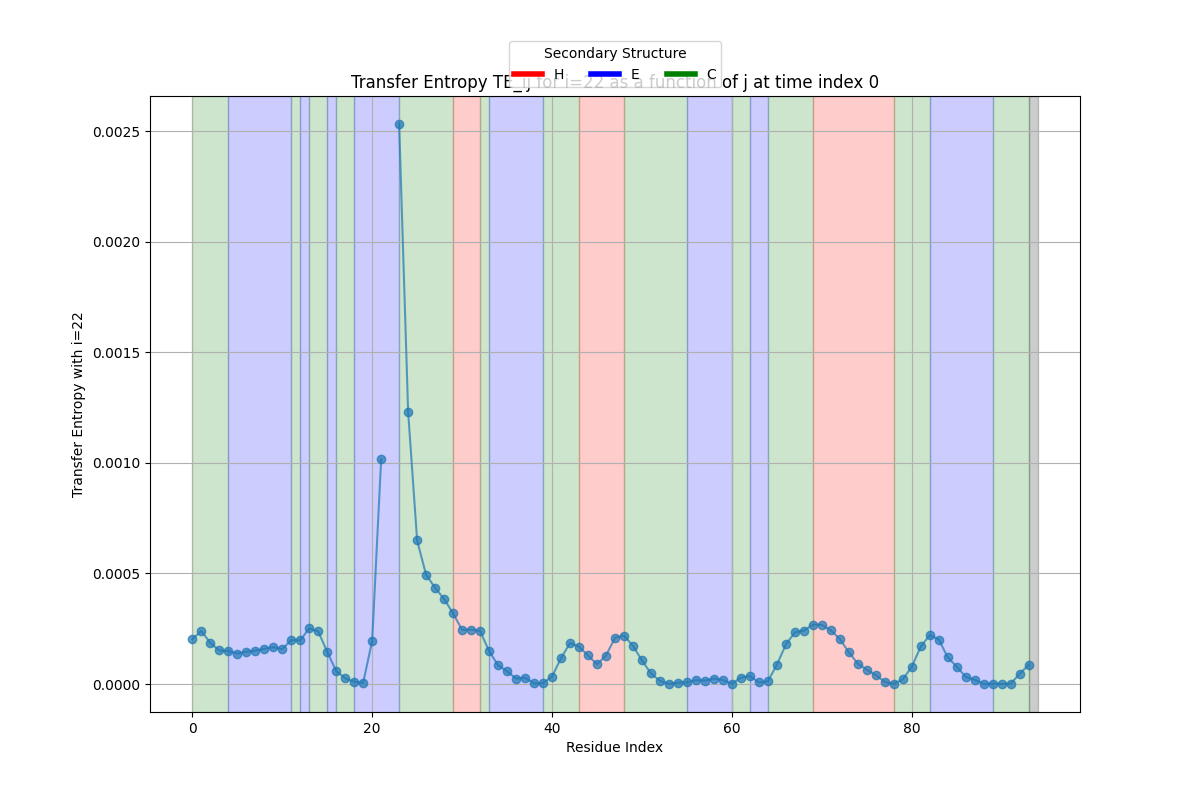
\includegraphics[width=0.5\textwidth]{images/3LNXTransfer Entropy TE_ij for i=22 as a function of j at time index 0.png}
    \caption{Transfer Entropy}
\end{figure}
\section{3LNY}
\begin{figure}[h]
    \centering
    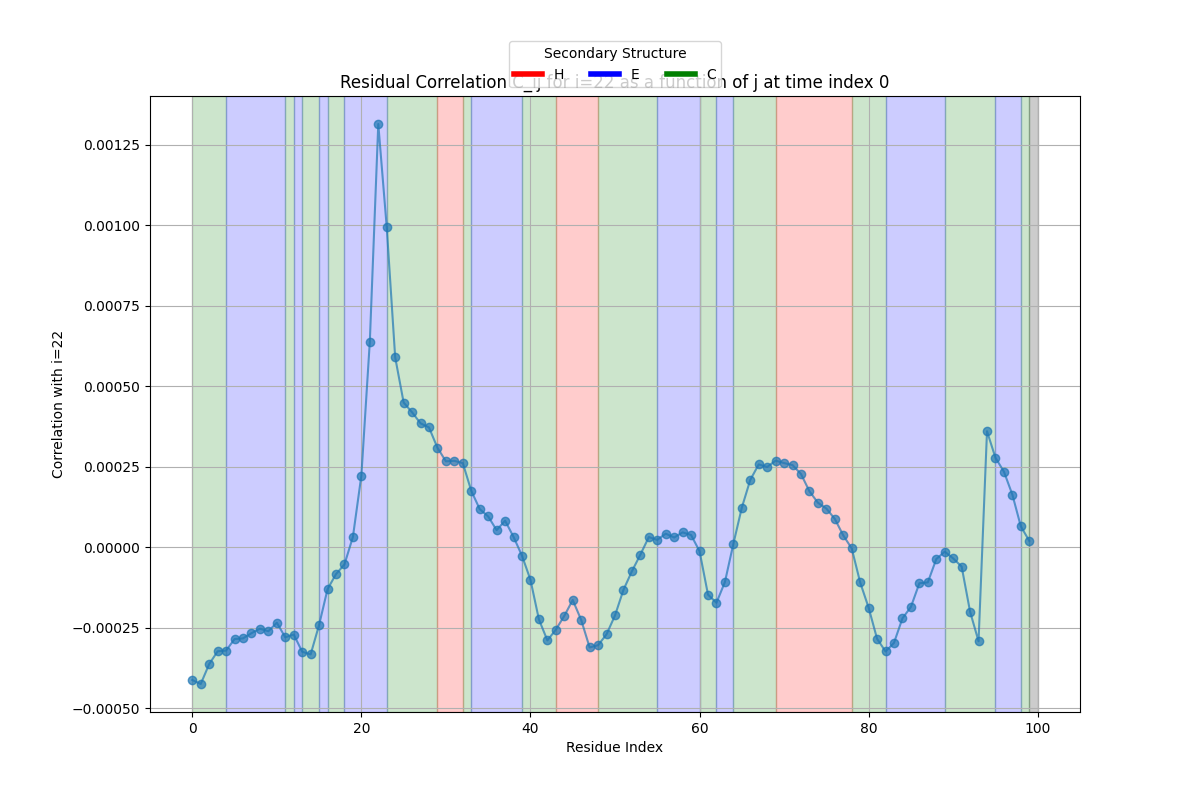
\includegraphics[width=0.5\textwidth]{images/3LNYResidual Correlation C_ij for i=22 as a function of j at time index 0.png}
    \caption{Correlazione}
\end{figure}
\begin{figure}[h]
    \centering
    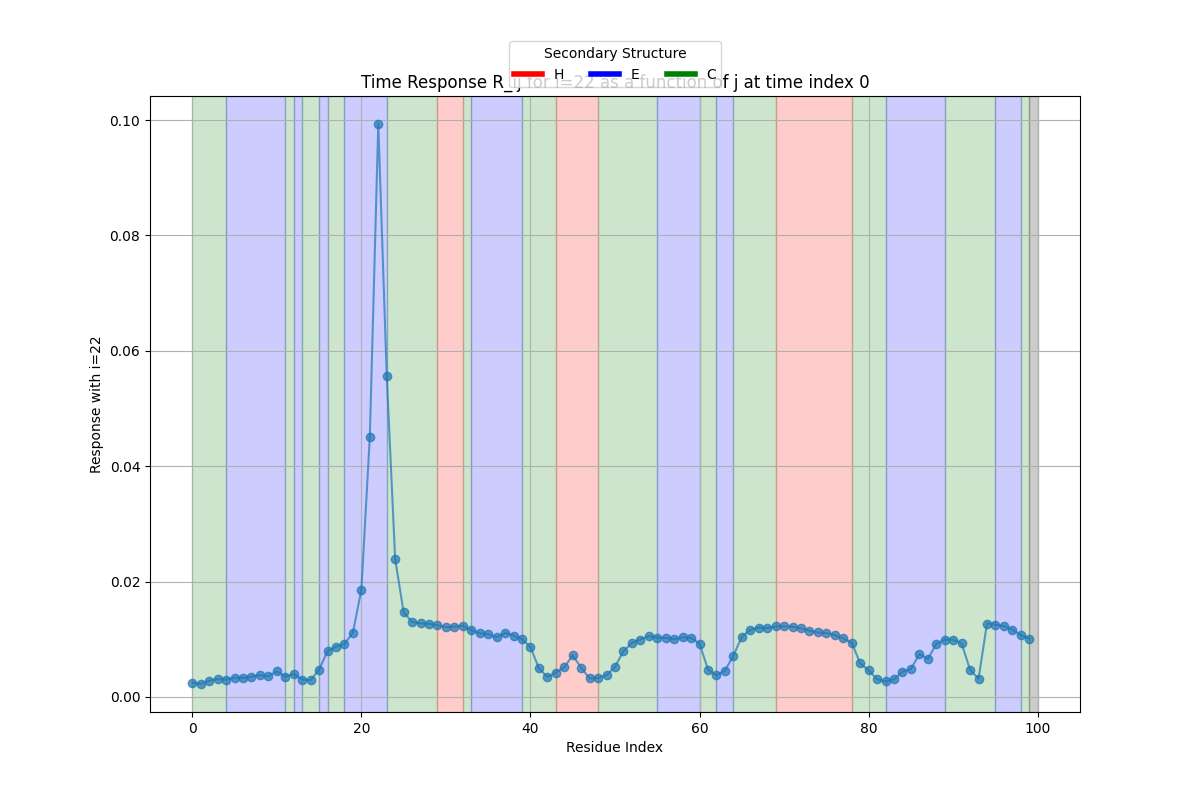
\includegraphics[width=0.5\textwidth]{images/3LNYTime Response R_ij for i=22 as a function of j at time index 0.png}
    \caption{Risposta}
\end{figure}

\begin{figure}[h]
    \centering
    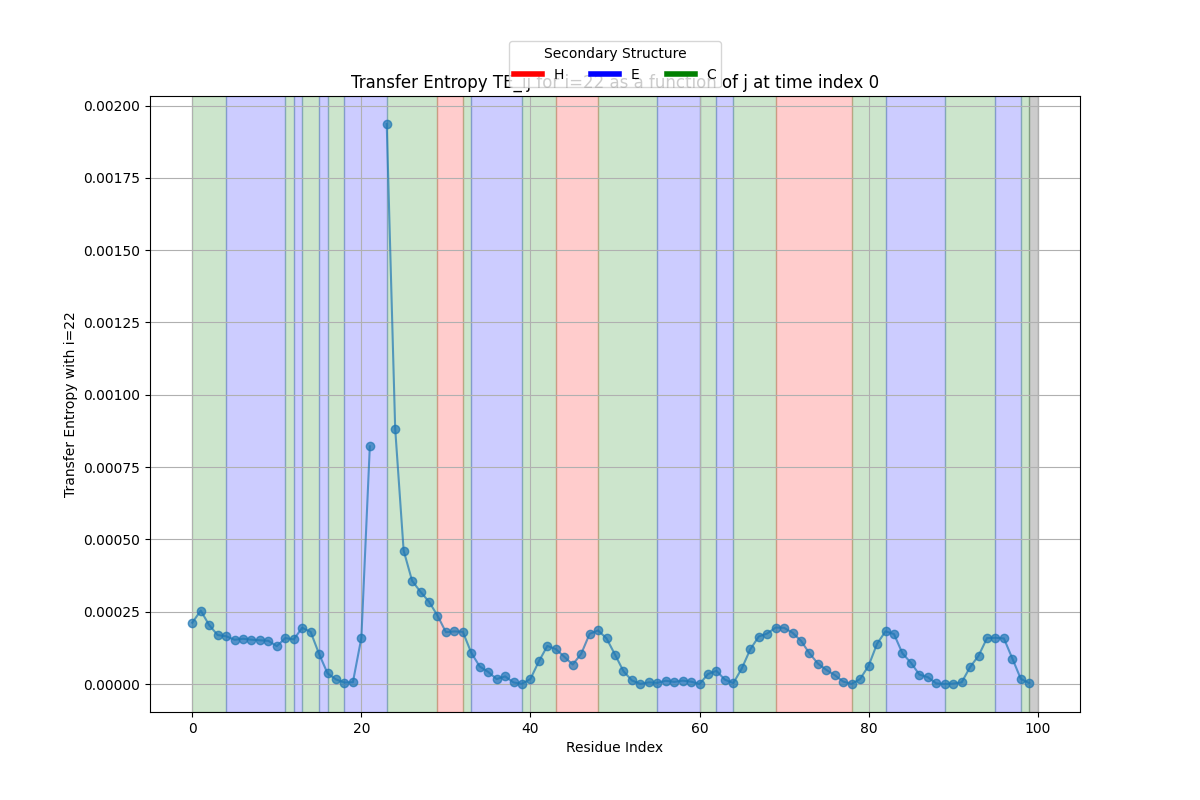
\includegraphics[width=0.5\textwidth]{images/3LNYTransfer Entropy TE_ij for i=22 as a function of j at time index 0.png}
    \caption{Transfer Entropy}
\end{figure}
\end{document}